\documentclass{article}

\usepackage{graphicx} % Required for the inclusion of images
\usepackage{natbib} % Required to change bibliography style to APA
\usepackage{amsmath} % Required for some math elements 

\setlength\parindent{0pt} % Removes all indentation from paragraphs

\renewcommand{\labelenumi}{\alph{enumi}.} % Make numbering in the enumerate environment by letter rather than number (e.g. section 6)

%\usepackage{times} % Uncomment to use the Times New Roman font
\usepackage{hyperref}
\usepackage{listings}
\usepackage{caption}
\usepackage{subcaption}


%----------------------------------------------------------------------------------------
%	DOCUMENT INFORMATION
%----------------------------------------------------------------------------------------
\title{Scientific Visualization \\ Excersise Report}
\author{Denys \textsc{Sobchyshak}}
\date{January 30, 2015}

\begin{document}
\maketitle

\section{ImageVis 3D}
In the first part of the exercise we got acquainted with an ImageVis 3D volume rendering tool and tried to perform several simple visualizations of various data sets using it. Along the way we learned several different volume rendering options, namely: direct volume and iso-surface rendering, clear view mod and we also used a color transfer function to obtain specific visualizations that we wanted.

\subsection{$\text{C}_{60}$ Molecule}
First data set represented fullerene, carbon molecule in the shape of a hollow sphere. Our base, non-filtered data looked like a gray iso-surface depicted on figure \ref{fig:base}. While investigating various features of color transfer we found a way to visualize inner structure of the molecule, specifically its atoms and their bondings, which is depicted in figure \ref{fig:bondings}. I've also managed to visualize both the atoms with bondings and molecule centers as depicted on figure \ref{fig:2ndview}. All of this was achieved by figuring out which part of transfer functions (in essence, which part of data) was responsible for specific volumes and then only tuning the values, results of which you can find on figure \ref{fig:2}.

\begin{figure}
	\centering
	\begin{subfigure}[h]{0.2\textwidth}
		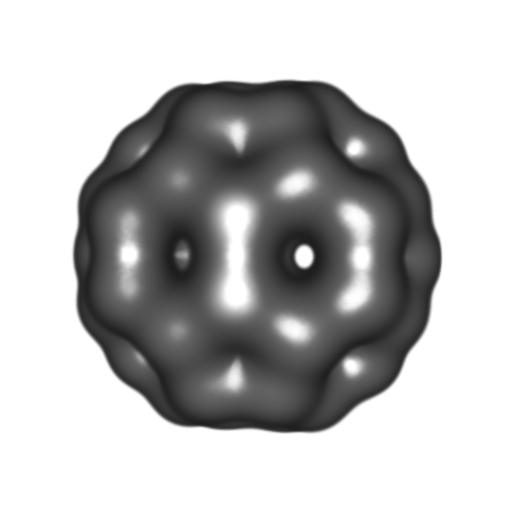
\includegraphics[width=\textwidth]{base-vis.png}
		\caption{Non-filtered data}
		\label{fig:base}
	\end{subfigure}
	\begin{subfigure}[h]{0.2\textwidth}
		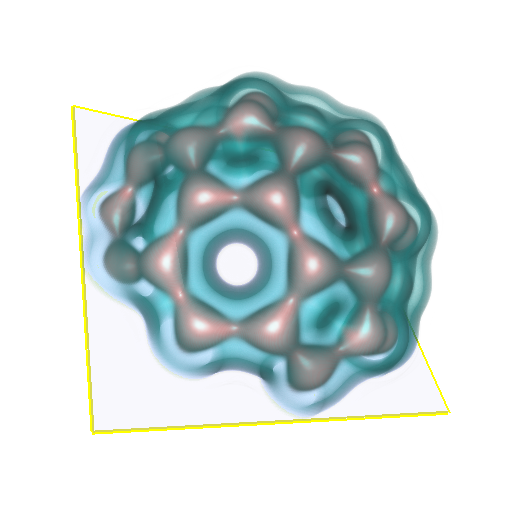
\includegraphics[width=\textwidth]{bondings.png}
		\caption{Atoms and bondings}
		\label{fig:bondings}
	\end{subfigure}
	\begin{subfigure}[h]{0.2\textwidth}
		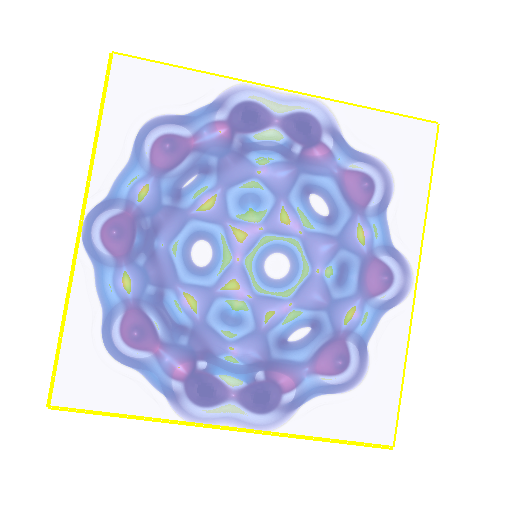
\includegraphics[width=\textwidth]{crosscut.png}
		\caption{Molecule crosscut}
		\label{fig:crosscut}
	\end{subfigure}
	\begin{subfigure}[h]{0.2\textwidth}
		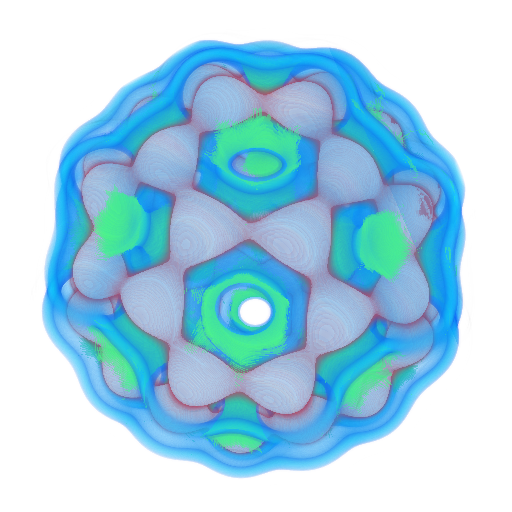
\includegraphics[width=\textwidth]{2d-view.png}
		\caption{Non-filtered data}
		\label{fig:2ndview}
	\end{subfigure}
	\caption{$\text{C}_{60}$ Visualization}\label{fig:1}
\end{figure}
\begin{figure}
	\centering
	\begin{subfigure}[h]{0.45\textwidth}
		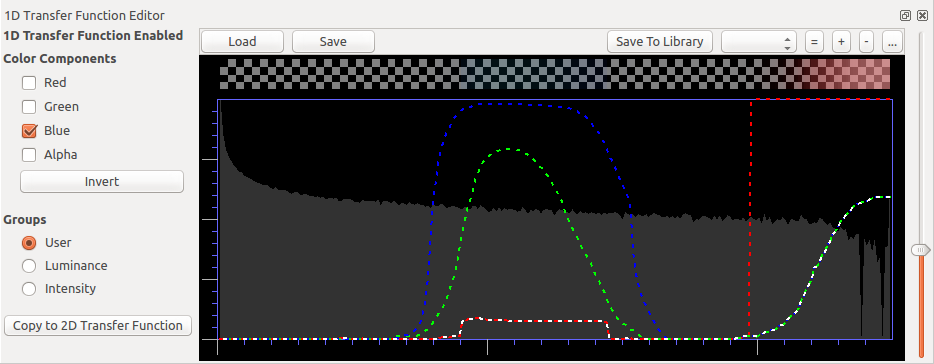
\includegraphics[width=\textwidth]{1d-transfer.png}
		\caption{1D}
		\label{fig:1dt}
	\end{subfigure}
	\begin{subfigure}[h]{0.45\textwidth}
		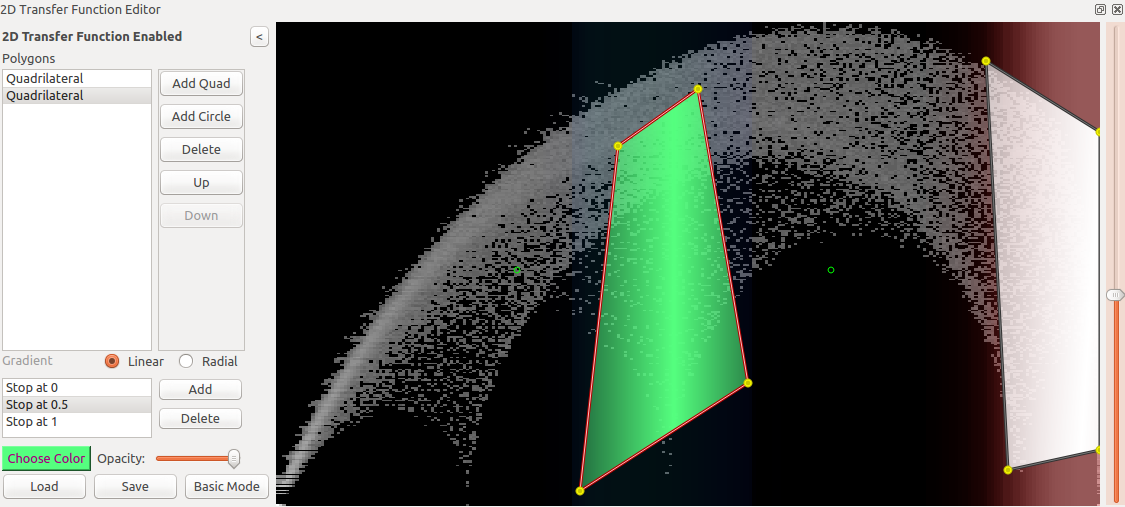
\includegraphics[width=\textwidth]{2d-trasfer.png}
		\caption{2D}
		\label{fig:2dt}
	\end{subfigure}
	\caption{Transfer functions used to visualize $\text{C}_{60}$ Molecule}\label{fig:2}
\end{figure}

However, a simpler approach to these tasks was to just visualize isosurface with clear-view mod enabled as depicted on figure \ref{fig:3}.
\begin{figure}[h!]
	\begin{center}
		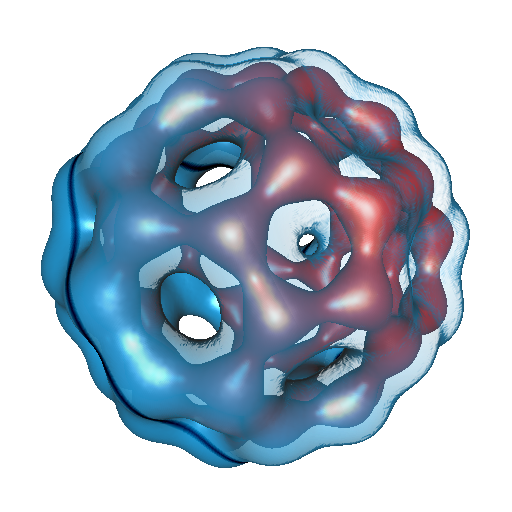
\includegraphics[width=0.2\textwidth]{isosurface.png}
		\caption{Isosuface of the Molecule}
		\label{fig:3}
	\end{center}
\end{figure}


\subsection{Engine}
Next data set represented some sort of engine with some inner parts. Among all trials the best looking visualization was accomplished using isosurfacing paired with clear-view mode depicted on figure \ref{fig:4} with its settings included.
\begin{figure}
	\centering
	\begin{subfigure}[h]{0.5\textwidth}
		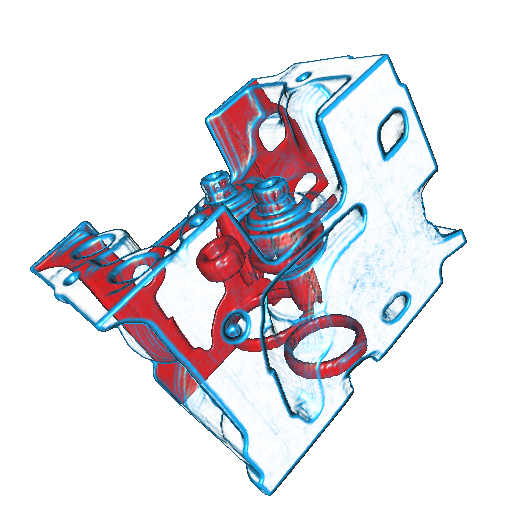
\includegraphics[width=\textwidth]{engine-iso-view.png}
		\caption{Isosurfacing}
		\label{fig:picture}
	\end{subfigure}
	\begin{subfigure}[h]{0.3\textwidth}
		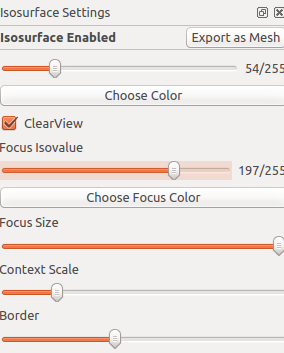
\includegraphics[width=\textwidth]{engine-isosurface.png}
		\caption{Settings}
		\label{fig:settings}
	\end{subfigure}
	\caption{Engine visualization}\label{fig:4}
\end{figure}

\subsection{Human head}
Another data set represented a detailed model of human head. This visualization was rather tricky since it was too complex to be used in pair with isosurfacing or 1D color transfer, thus I had to play quite a bit with 2D color transfer in order to have clear visualization of the skull and skin around it as depicted on figure \ref{fig:5}.
\begin{figure}
	\centering
	\begin{subfigure}[h]{0.45\textwidth}
		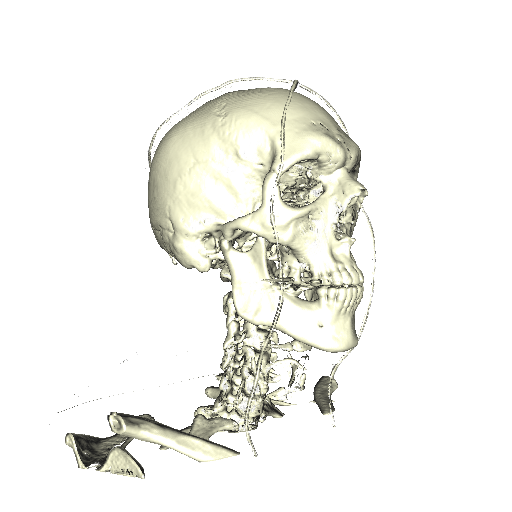
\includegraphics[width=\textwidth]{skeleton.png}
		\caption{The Scull}
		\label{fig:skeleton}
	\end{subfigure}
	\begin{subfigure}[h]{0.45\textwidth}
		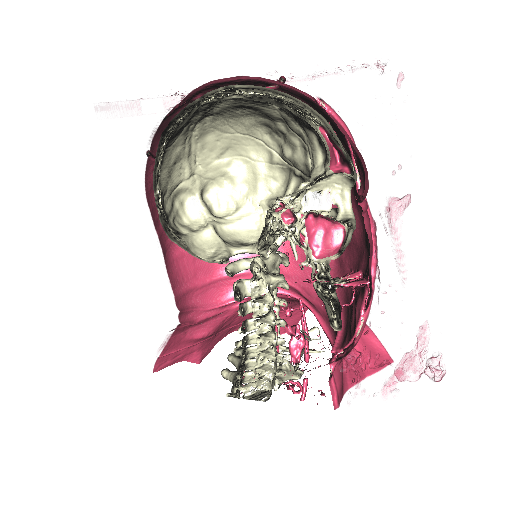
\includegraphics[width=\textwidth]{skel-surf.png}
		\caption{Scull with surrounding skin}
		\label{fig:skin}
	\end{subfigure}
	\caption{Human head visualization}\label{fig:5}
\end{figure}

\subsection{Piggy Bank}
The final data set represented a piggy bank. I've applied known by now 1D transfer function as depicted on figure \ref{fig:6} along with results of visualization. I've also visualized just the piggy with coins inside as depicted on figure \ref{fig:pigiso}. The tricky part of this data set was to figure out on 1D color transfer function which data corresponded to which volume, even with given data intensity graph.
\begin{figure}
	\centering
	\begin{subfigure}[h]{0.3\textwidth}
		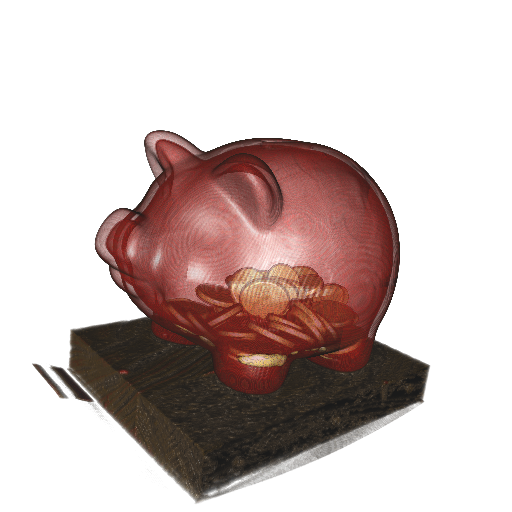
\includegraphics[width=\textwidth]{pig-1dvolren.png}
		\caption{Sample rendering}
		\label{fig:basepig}
	\end{subfigure}
	\begin{subfigure}[h]{0.3\textwidth}
		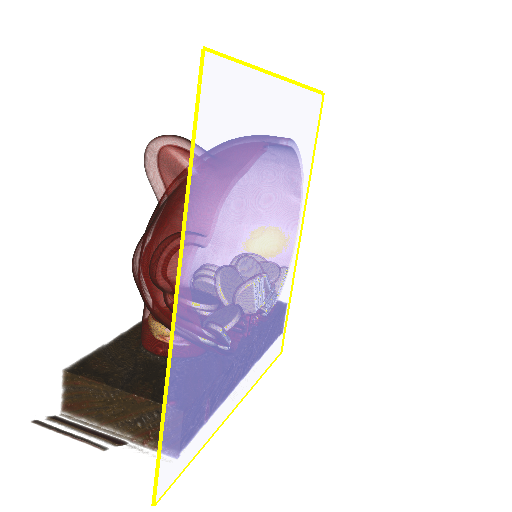
\includegraphics[width=\textwidth]{pig-clearcut.png}
		\caption{Cross cut}
		\label{fig:cut}
	\end{subfigure}
	\begin{subfigure}[h]{0.5\textwidth}
		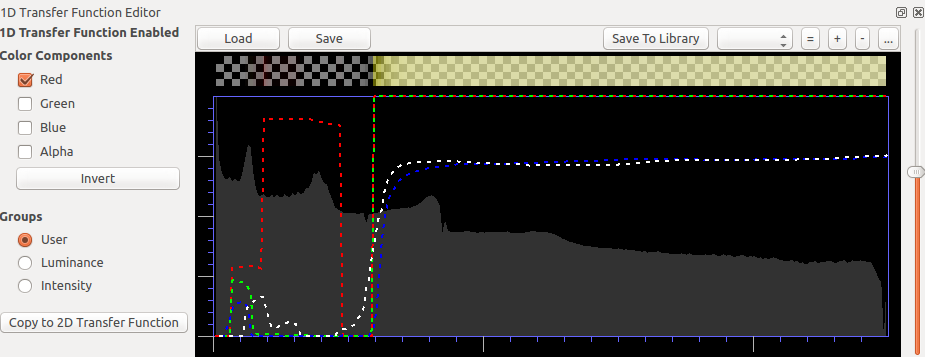
\includegraphics[width=\textwidth]{pig-1dt.png}
		\caption{Cross cut}
		\label{fig:1dtf}
	\end{subfigure}
	\begin{subfigure}[h]{0.3\textwidth}
		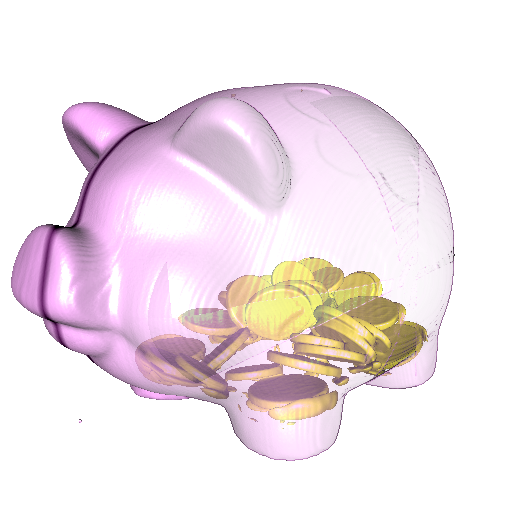
\includegraphics[width=\textwidth]{pig-isolines.png}
		\caption{Isosurfacing}
		\label{fig:pigiso}
	\end{subfigure}
	\caption{Piggy Bank Visualization}\label{fig:6}
\end{figure}


\section{ParaView}
In the second part of our exercise we got acquainted with ParaView, an advanced data analysis and visualization tool.

\subsection{Asian Dragon}
We started off with downloading and visualizing a rather detailed and complex model of an Asian dragon as depicted in figure \ref{fig:7}.
\begin{figure}
	\centering
	\begin{subfigure}[h]{0.4\textwidth}
		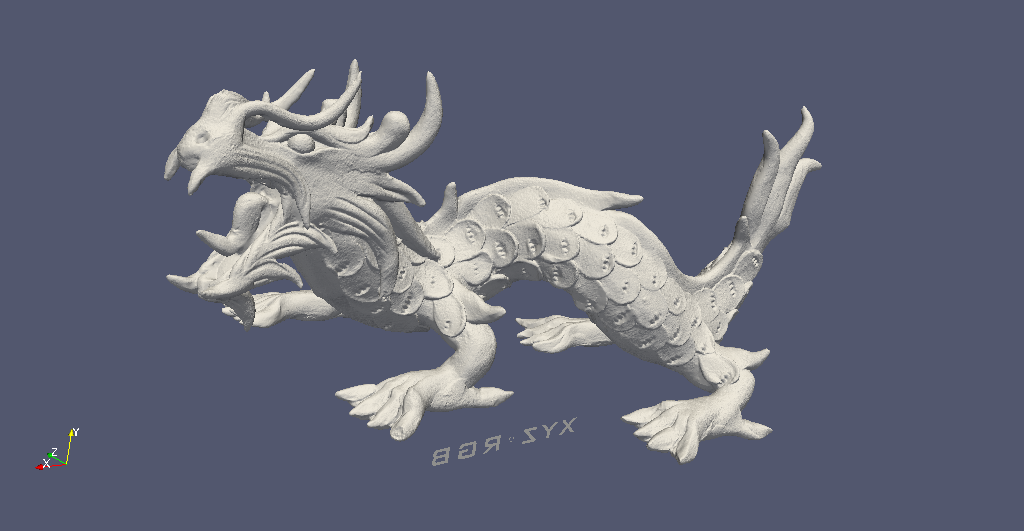
\includegraphics[width=\textwidth]{dragon.png}
		\caption{Base rendering}
		\label{fig:drake}
	\end{subfigure}
	\begin{subfigure}[h]{0.4\textwidth}
		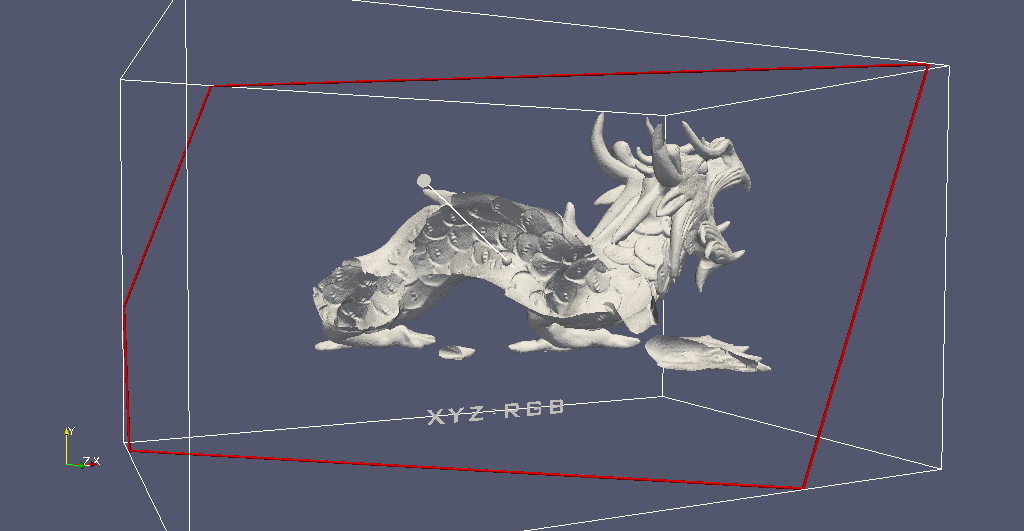
\includegraphics[width=\textwidth]{drugon-cut.png}
		\caption{Cross cut}
		\label{fig:drakecut}
	\end{subfigure}
	\caption{Asian dragon visualization}\label{fig:7}
\end{figure}

\subsection{Vector fild}
For this task we had to find vector field data set and visualize it. I've used data that was provided for a CFD course to simulated a 3D flow of water over cavity. Results of streamline and glyph visualization of velocity field can be found on figure \ref{fig:8}.
\begin{figure}
	\centering
	\begin{subfigure}[h]{0.45\textwidth}
		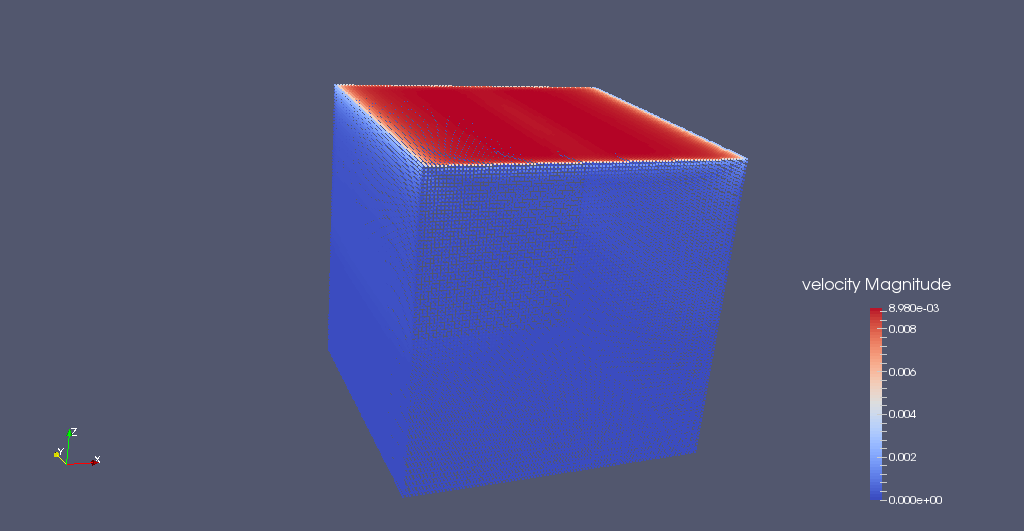
\includegraphics[width=\textwidth]{3d-cavity.png}
		\caption{Base cavity}
		\label{fig:cavbase}
	\end{subfigure}
	\begin{subfigure}[h]{0.45\textwidth}
		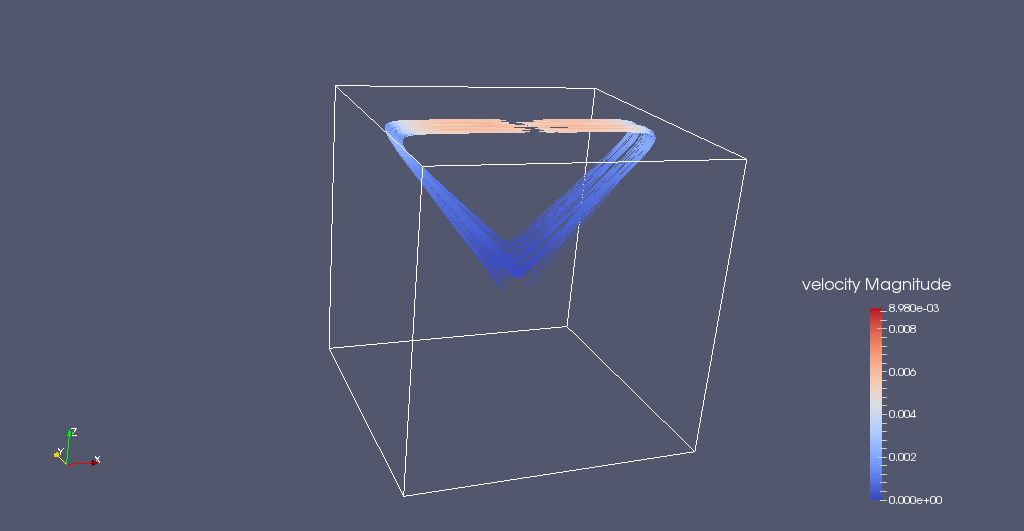
\includegraphics[width=\textwidth]{3d-cavity-streamlines.png}
		\caption{Streamline filter}
		\label{fig:strmlines}
	\end{subfigure}
	\begin{subfigure}[h]{0.6\textwidth}
		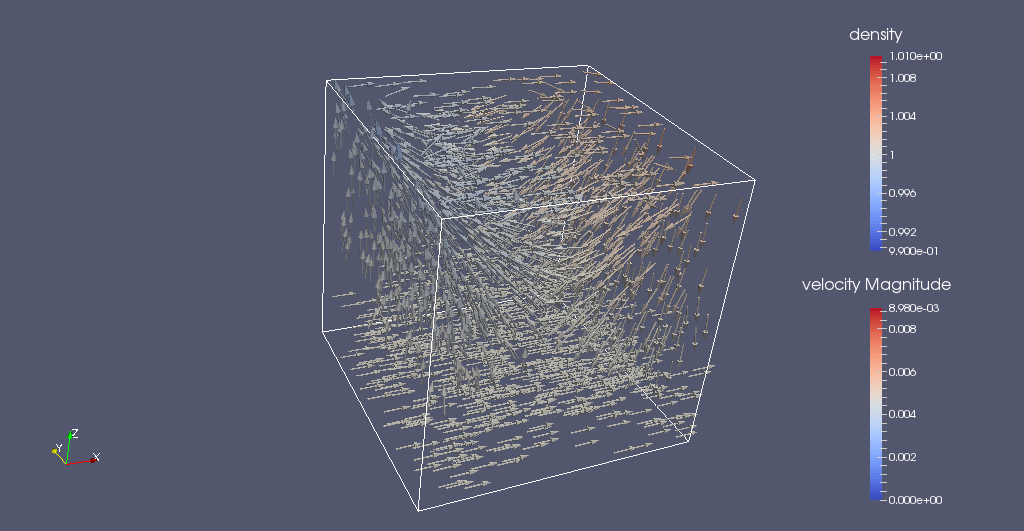
\includegraphics[width=\textwidth]{3d-cavity-glyph.png}
		\caption{Glyph filter}
		\label{fig:glyph}
	\end{subfigure}
	\caption{3D flow over cavity visualization}\label{fig:8}
\end{figure}

\subsection{PDB}
And the final part consisted of picking interesting data sets from \url{pdb.org}, visualizing them and comparing results to their online visualization. I've chosen next data:
\begin{enumerate}
	\item \textit{2XUA} - CRYSTAL STRUCTURE OF THE ENOL-LACTONASE FROM BURKHOLDERIA XENOVORANS LB400
	\item \textit{3T1Y} - Structure of the Thermus thermophilus 30S ribosomal subunit complexed with a human anti-codon stem loop (HASL) of transfer RNA Lysine 3 (TRNALYS3) bound to an mRNA with an AAG-codon in the A-site and paromomycin
\end{enumerate}
with their comparative visualization given in figure \ref{fig:9} and \ref{fig:10}.

\begin{figure}
	\centering
	\begin{subfigure}[h]{0.3\textwidth}
		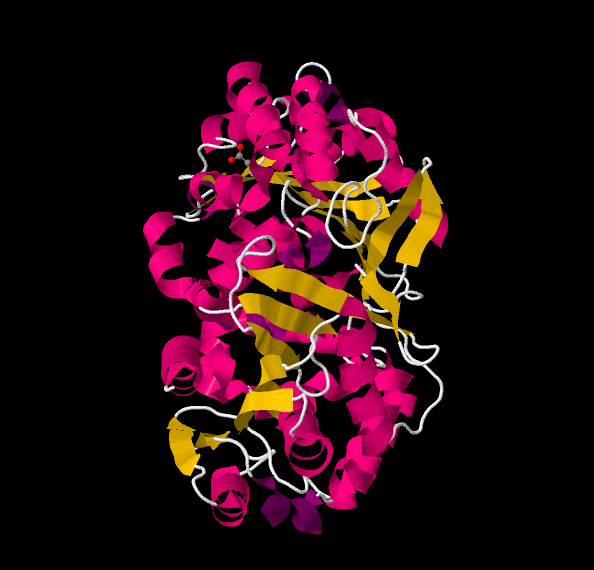
\includegraphics[width=\textwidth]{pdb-2xua.png}
		\caption{PDB Viewer}
		\label{fig:pdb1}
	\end{subfigure}
	\begin{subfigure}[h]{0.5\textwidth}
		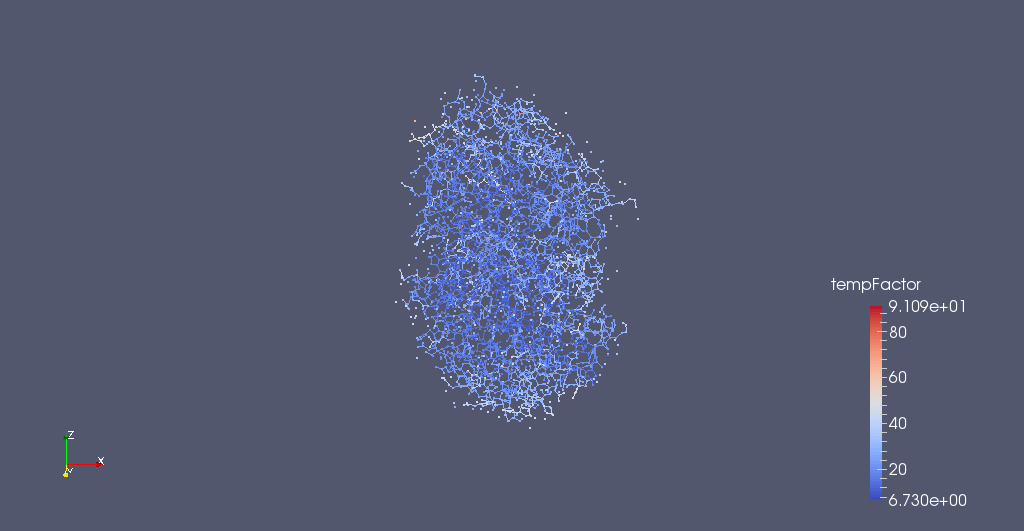
\includegraphics[width=\textwidth]{2xua.png}
		\caption{ParaView}
		\label{fig:pv}
	\end{subfigure}
	\caption{2XUA visualization}\label{fig:9}
\end{figure}

\begin{figure}
	\centering
	\begin{subfigure}[h]{0.3\textwidth}
		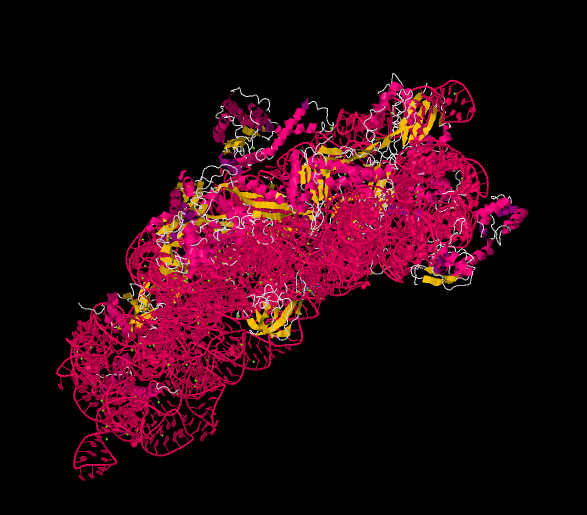
\includegraphics[width=\textwidth]{pdb-3t1y.png}
		\caption{Base cavity}
		\label{fig:pdb2}
	\end{subfigure}
	\begin{subfigure}[h]{0.5\textwidth}
		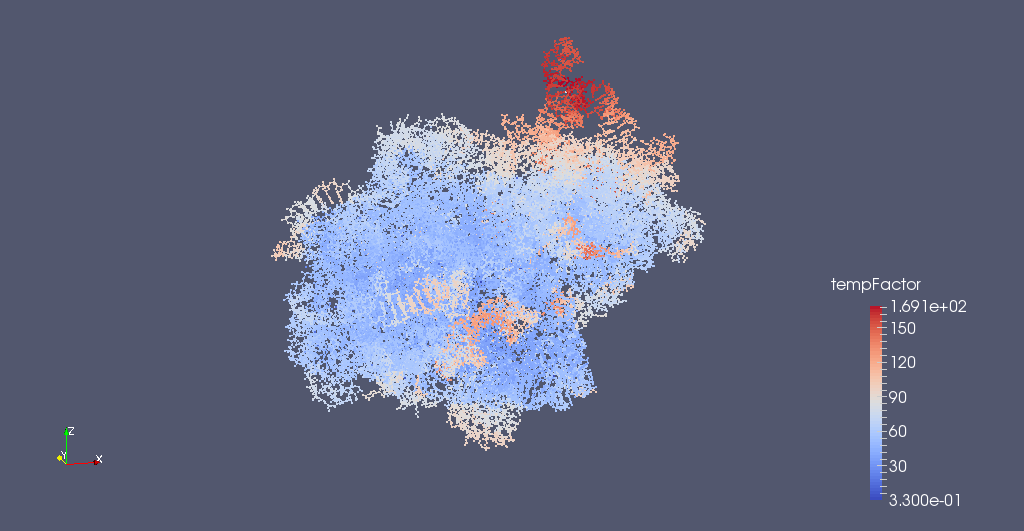
\includegraphics[width=\textwidth]{3t1y.png}
		\caption{ParaView}
		\label{fig:pv2}
	\end{subfigure}
	\caption{3T1Y visualization}\label{fig:10}
\end{figure}

Even though I couldn't find a way to make visualization in paraview look any close to how it looks at \url{pdb.org}, one can notice that general structure of molecules remains the same leading us to believe that ParaView is not the best tool to visualize such data. However, in my experience it is a very useful tool for engineering applications and it provides rather vast amount of various filters and visualization options which make it quite flexible and adaptable for a big number of purposes.


%----------------------------------------------------------------------------------------
\end{document}